\documentclass{sig-alternate-05-2015}

\usepackage{multirow}
\usepackage{color}
\usepackage{algorithm}
\usepackage{algorithmic}
\DeclareMathOperator*{\argmin}{argmin}
\DeclareMathOperator*{\argmax}{argmax}

\newcommand{\cheng}[1]{\textcolor{green}{\textbf{Cheng: }{\footnotesize #1}}}
\newcommand{\lexing}[1]{\textcolor{red}{\textbf{Lexing: }{\footnotesize #1}}}
\newcommand{\dawei}[1]{\textcolor{blue}{\textbf{Dawei: }{\footnotesize #1}}}

\newcommand{\etal}{{\em et al.}\xspace}
\usepackage{url}
\usepackage{hyperref}
\newcommand{\surl}[1]
{
	\urlstyle{same}\url{#1}
}

\usepackage[svgnames]{xcolor}
\definecolor{navy}{rgb}{0.1, 0.1, 0.8}
\definecolor{gray}{rgb}{0.4, 0.4, 0.4}

\newcommand{\eat}[1]{}
\newcommand{\rev}[1]{{\color{navy}{#1}}}
\newcommand{\verify}[1]{{\color{red}{#1}}}
\usepackage{soul} %% needed for highlighting
\newcommand{\TODO}[2]{ { [{\bf #1}:~{\hl{#2}}]}}

% place holder spacing hacks
\newcommand{\secmoveup}{\vspace{-0.0mm}}                %{\vspace{-0.12in}}
\newcommand{\bigsecmoveup}{\secmoveup\vspace{-.0mm}}   %{\vspace{-0.08in}}
\newcommand{\textmoveup}{\vspace{-0.mm}}               %{\vspace{-0.08in}}
\newcommand{\bigtextmoveup}{\textmoveup\vspace{-0.0in}} %{\vspace{-0.06in}}
\newcommand{\itemmoveup}{\vspace{-0mm}}              %{\vspace{-0.04in}}
\newcommand{\eqmoveup}{\vspace{-0.0in}}                 %{\vspace{-0.16in}}
\newcommand{\captionmoveup}{\eqmoveup\vspace{-0.0in}}   %{\vspace{-0.16in}}
\newcommand{\refitemmoveup}{\vspace{-0mm}}            %{\vspace{-0.16in}}

\begin{document}

%\setcopyright{}
%\doi{}
%\isbn{}
%\conferenceinfo{}
%\acmPrice{\$15.00}
% Author Metadata

%\title{Recommending Trajectories by Ranking Points of Interest and Structured Prediction}
%\title{Learning Ranks and Routes for Tour Recommendation}
\title{Learning Ranks and Routes to Recommend Trajectories}
%\title{Structured Prediction for Trajectory Recommendation}

%\numberofauthors{3}
%\author{
%    \alignauthor Dawei Chen$^{*\dagger}$\\
%    \alignauthor Cheng Soon Ong$^{*\dagger}$\\
%    \alignauthor Lexing Xie$^{*\dagger}$\\
%    \and
%    $^*$The Australian National University, $^\dagger$Data 61, CSIRO, Australia\\
%    \and
%    \{u5708856, chengsoon.ong, lexing.xie\}@anu.edu.au
%}

% The code below should be generated by the tool at
% http://dl.acm.org/ccs.cfm
% Please copy and paste the code instead of the example below.
\begin{CCSXML}
    <ccs2012>
    <concept>
    <concept_id>10002951.10003317.10003347.10003350</concept_id>
    <concept_desc>Information systems~Recommender systems</concept_desc>
    <concept_significance>500</concept_significance>
    </concept>
    <concept>
    <concept_id>10002951.10003227.10003233.10010519</concept_id>
    <concept_desc>Information systems~Social networking sites</concept_desc>
    <concept_significance>300</concept_significance>
    </concept>
    </ccs2012>
\end{CCSXML}
\ccsdesc[500]{Information systems~Recommender systems}
\ccsdesc[300]{Information systems~Social networking sites}

\maketitle

\begin{abstract}
Recommending Points of Interest (POIs) and trajectories to tourists by exploring data with 
geographical information from on-line social media is an interesting and challenging task.
We propose to utilize learning to rank and Markov Chain to capture the properties of POIs
as well as the transition pattern between POIs, transition probabilities between POIs were
factorized according to several POI features to deal with data sparsity.
Furthermore, a probabilistic model and a structured support vector machine were leveraged 
to combine the results of learning to rank as well as the Markov Chain to recommend trajectories.
Experimental results on four trajectory datasets extracted from Flickr photos show performance 
improvements of our approach over the state-of-the-art and reveal many interesting properties 
of trajectories in different datasets.

\end{abstract}

\keywords{Trajectory recommendation, Learning to rank, Planning}

%!TEX root = main.tex

\section{Introduction}
\label{sec:intro}

This paper proposes a novel solution to recommend travel routes in cities.
Large amount of location traces are becoming available from ubiquitous location tracking devices.
For example FourSquare, the local search and discovery service, has 50 million monthly users who have made 8 billion check-ins~\cite{4sq}; Flickr, the online photo-sharing site, hosts over 2 billion geo-tagged public photos~\cite{flickr}. Such large amounts of travel data provides new opportunities for better
travel planning traditionally done with written travel guides,
choosing and ranking locations for a variety of activities from dining to recreation,
and potential new solutions to orienteering and routing problems.
Good solutions to these problems will in turn lead to better urban experiences for residents and visitors alike, and foster sharing of even more location-based behaviour data.

There are several settings of recommendation problems for locations and routes: POI recommendation,
next location recommendation, and trajectory recommendation. This is described in more detail in
Section~\ref{sec:relatedwork}, and we refer the reader to a number of recent
surveys\cite{bao2015recommendations,zheng2015trajectory,zheng2014urban}
for detailed profiles of the area.
We propose a novel way to learn point and route preferences jointly.
Our solution consists of several parts.
We propose a learning to rank formulation to capture the preference of POIs given the starting and ending points of a trajectory (Section~\ref{sec:method}).
We model pair-wise transition patterns between POIs by factorising the transition likelihoods along five different types of location properties,
which alleviates data sparsity between each pair of POIs and allows POIs of the same type and neighborhood to share parameters.
We combine the results of point and transition ranking using Markov chain inference and route planning techniques (Section~\ref{sec:recommendation}). We further propose a novel way to jointly learn point and transition scores with a Structured Support Vector Machine (StructuredSVM). In Section~\ref{sec:experiment},
we evaluate the proposed algorithms on photo trajectories in five different cities, with a traditional metric $F_1$ on POIs as well as a novel pairs-$F_1$ metric specifically designed for trajectories.

The main contributions of this work is as follows:
\begin{itemize}
\setlength{\itemsep}{-2pt}
\item We propose a novel algorithm to jointly optimise point preference and route plan.
  We find that the learning-based approaches generally out-perform heuristic route recommendation~\cite{ijcai15}. Incorporating transitions to POI ranking improves the pairs-$F_1$ metric for correct sequences of POIs, and that routing algorithms that disallow sub-tours generally out-perform Markov chain methods.
\item Our approach is feature-driven and learns from past behaviour without having to design specialised treatment for spatial, temporal and social information. It currently incorporates information about location, POI categories and behaviour history, and can use additional social or time information.% as long as they are  encoded in features.
\item We show good performance compared to recent results~\cite{ijcai15}, and also quantify the contribution from the different components, such as point ranking, scoring transitions, and routing.
\item We propose a new metric to evaluate trajectories: pairs-$F_1$, which has the property of being between 0 and 1, and being 1 if and only if two trajectories are exactly the same. Our benchmark data and results are publicly available.
\end{itemize}

\begin{figure*}[ht]
	\centering
	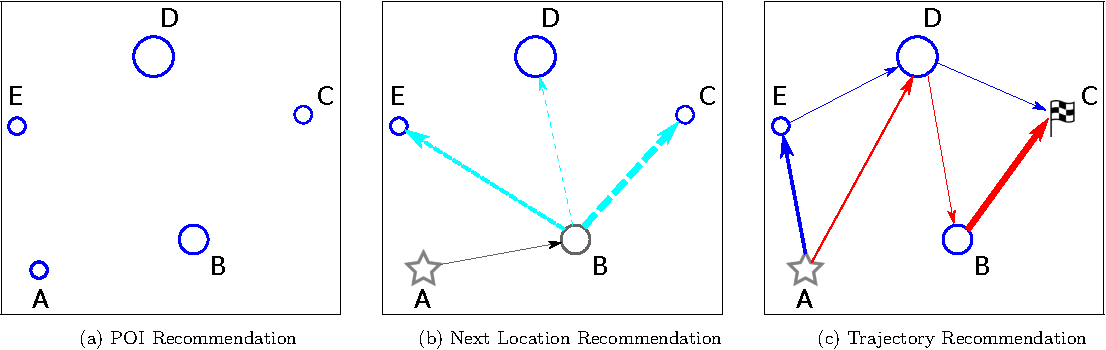
\includegraphics[width=0.7\textwidth]{fig/fig1-flavours.pdf}
	\caption{Three settings of trajectory recommendation problems: (a) POI recommendation, (b) next location recommendation, and (c) trajectory recommendation. Node size: POI score; edge width: transition score between pairs of POIs; grey: input query; star: starting location; flag: ending location. See the second paragraph of Section~\ref{sec:intro} for details.
}
	\label{fig:threesettings}
\end{figure*}



%!TEX root = main.tex

\section{Related Work}
\label{sec:relatedwork}


\begin{figure*}[htbp]
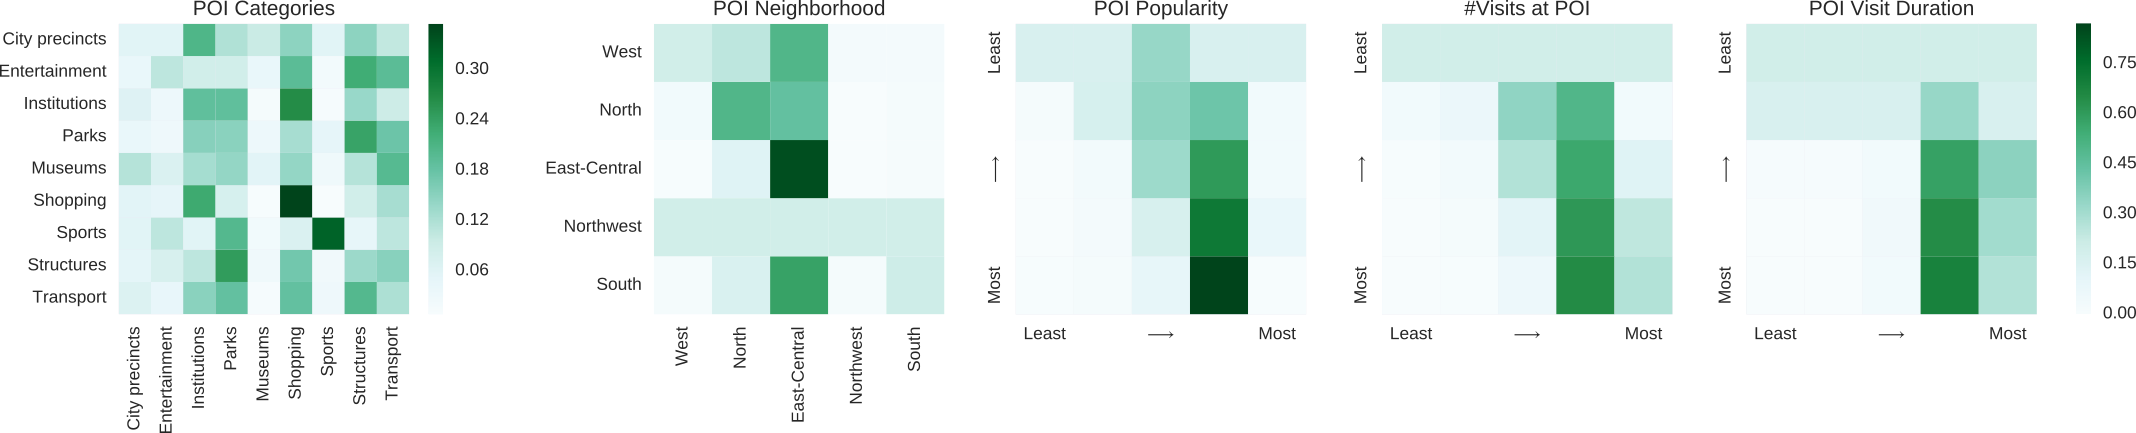
\includegraphics[width=\textwidth]{fig/poi_transmat.png}
\caption{Transition matrices for $5$ individual POI features (Melbourne)}
\label{fig:transmat}
\end{figure*}



%As geo-tagged travel data become widely available, problems in exploring routes and travel patterns has received increasing attention across several research communities -- including information retrieval and recommender systems, databases, social media, geographic information systems, and artificial intelligence.
%Exhaustive surveying of the area is beyond the scope of this work, we refer the readers to a number of
We summarise recent work most related to formulating and solving learning problems on assembling routes
from points-of-interest (POI), according to the problem setting, the method for ranking places and routes, as well as the use of different features and queries.

{\bf Problem settings} for travel patterns and trajectory data.
There are several settings of recommendation problems for locations and routes, as illustrated in Figure~\ref{fig:threesettings}.
The first setting can be called points-of-interest (POI) recommendation (Figure~\ref{fig:threesettings}(a)). Each location (A to E) is scored with geographic and behavioural information such as category, reviews, popularity, spatial information such as distance, and temporal information such as travel time uncertainty, time of the day or day of the week.
This can be in discovery mode, such as identifying points-of-interest~\cite{zheng2009mining,li2015instagram} and includes efficient querying of geographic objects for trips ~\cite{hashem2015efficient}
A popular approach is based on the collaborative filtering model
for learning user-location affinity~\cite{shi2011personalized}, with additional ways to incorporate spatial~\cite{lian2014geomf,liu2014exploiting}, or temporal~\cite{yuan2013timeaware,hsieh2014mining,gao2013temporal}, or spatial-temporal~\cite{yuan2014graph} information.
There is a rich collection of recent literature on this problem~\cite{yin2015joint,shi2011personalized,lian2014geomf,liu2014exploiting,yuan2013timeaware,hsieh2014mining,gao2013temporal,yuan2014graph}, including recent surveys~\cite{bao2015recommendations,zheng2014urban}.


Figure~\ref{fig:threesettings}(b) illustrates the second setting: next location recommendation~\cite{ijcai13,aaai16,baraglia2013learnext,zhang2015location}. Here the input is a partial trajectory (e.g. started at point A and currently at point B), the task of the algorithm is to score the next candidate location (e.g, C, D and E) based on the perceived POI score and transition compatibility with input $A\rightarrow B$.
It is a variant of POI recommendation except given both the user and locations travelled to date. The solutions to this problem include incorporating Markov chains into collaborative filtering~\cite{fpmc10,ijcai13,zhang2015location},
quantifying tourist traffic flow between points-of-interest~\cite{zheng2012patterns},
by formulating a binary decision or ranking problem~\cite{baraglia2013learnext}, or with sequence models such as recurrent neural networks~\cite{aaai16}.



This paper considers the final setting: route recommendation, as illustrated in Figure~\ref{fig:threesettings}(c). Here the input are some factors about the desired route, e.g. starting point A and end point C, along with auxiliary information such as the desired length of trip. The algorithm needs to take into account location desirability (as indicated by node size) and transition compatibility (as indicated by edge width), and compare route hypotheses such as A-D-B-C and A-E-D-C. Existing work in this area either uses heuristic combination of locations and routes~\cite{lu2010photo2trip,ijcai15,lu2012personalized}, or formulates an optimisation problem that is not informed or evaluated by behaviour history~\cite{gioniswsdm14,chen2015tripplanner}. Joint learning of locations preferences and routes remains an open problem.
Our work is in this category, we formulate a learning problem to score the whole trajectory, taking into account individual POI properties and relationships among different POIs.



%We group the methods for ranking and recommending location and trajectories into three broad categories.
{\bf Methods} for ranking locations and trajectories.
The first is collaborative filtering, or matrix factorisation family of techniques applied to places and trajectories~\cite{shi2011personalized,ijcai13,zhang2015location}. The second type regards route recommendation as a planning problem~\cite{gioniswsdm14,ijcai15}.
%Gionis et al~\cite{gioniswsdm14} formulates optimisation problems with additive user satisfaction and coverage constraints. Lim et al.~\cite{ijcai15} uses a combination of user preference and POI popularity as objective function, and then solves a travelling salesman problem (TSP) to obtain a route.
The TripBuilder system~\cite{brilhante2013shall} first solves a maximum coverage problem for user preference and then solves TSP for routing. The collaborative filtering approaches rank POI but do not take into account the sequence that a trip is taken. On the other hand, the planning approaches assume a fixed objective function that is not directly optimised to predict user behaviour. There have been a few approaches that jointly consider POI preference and routes~\cite{lu2012personalized, kurashima2010geotag,chen2015tripplanner}.
%Lu et al~\cite{lu2012personalized} uses heuristic combinations for point scoring, followed by branch-n-bound search for planning. Kurashima et al~\cite{kurashima2010geotag} modelled user preferences and his/her transition patterns between POIs using a hybrid of Markov chain and topic models, the search for a best path is done by greedily maximising the probability for the next point. The TripPlanner system~\cite{chen2015tripplanner} selects POIs based on input query and POI categories, and then scores routes using heuristic search strategies taking into account traffic and travel time constraints.
We propose a new approach that combines different POI features and POI-POI transition features, while learning the relevant weights from data. We also provide a comprehensive benchmark on how node- and edge- features contribute to the final trajectory ranking.


%planning:
%% Trip Builder
%\cite{tripbuilder15} recommended trajectories by first addressing a Generalized Maximum Coverage problem with respect to user preference and
%time budget to get a set of candidate trajectories, which were then scheduled by solving a variant of Traveling Salesman Problem to form the
%final recommendation.
%% WSDM'14
%\cite{gioniswsdm14} proposed a framework to recommend trajectories based on user provided constraints such as the visiting order of different
%categories of POIs, time and distance budget as well as the upper/lower bounds of the number of POIs in each category that a user wish
%to visit, user satisfaction at a POI was modeled by either associate a benefit or a set of other POIs and activities to that POI,
%and proved the maximization of user satisfaction is NP-hard in both cases.
%They further proposed pseudo polynomial dynamic programming algorithms as well as
%a $1-\epsilon$ approximation algorithm to maximize the user satisfaction.


%joint
%\cite{lu2012personalized} claims to do both point ranking and trip planning, heuristic combination for point scoring, branch-n-bound search for planning.
%% IJCAI'15
%Lim et al.~\cite{ijcai15} modeled user's interest on a specific category of POIs based on the observation that if a user is more interested in a certain category of POIs, his/her visit duration would be longer than the average visit duration in general. They then formulated trajectory recommendation as a Orienteering problem and use integer programming to optimize an objective which was a composite of the total POI popularity as well as the total user interest on POIs in the recommended trajectory
%with respect to a number of constraints such as the start/destination POI and time budget.
%\cite{kurashima2010geotag} modeled user preferences of POIs and his/her transition patterns
%between POIs using a hybrid of
%Markov and topic models, and recommend a trajectory by search the sequence of POIs with highest probability for %this user  with respect to a time budget.
%greedy on best next location.


%{\bf queries, features, available data}
%One of the challenges for modeling traveling behavior is the diversity of available information,
{\bf A diverse set of available information},
such as geographic, time, user properties, and subjective opinions.
Approaches for modelling space include geolocation-informed matrix factorisation~\cite{lian2014geomf}, spatial topic models~\cite{hu2013spatialtopic}, neighbourhood information~\cite{liu2014exploiting}, exploiting sequential information with additive Markov chain~\cite{zhang2014lore}, and enriching location with the information for venues~\cite{deveaud2014importance,deveaud2015experiments}.
Important variants to consider for modelling time include travel time~\cite{gao2013temporal},
constructing time-aware routes~\cite{yuan2013timeaware,hsieh2014mining}, time-of-day and day-of-week~\cite{chen2015tripplanner}, POI availability and uncertainty in travelling time~\cite{zhang2015personalized}. There are a number of approaches that jointly consider space and time\cite{yuan2014graph,zhang2015location}, such as modelling the correlation between check-in time and location~\cite{gao2013temporal}.
Inferring user attributes and preferences has been an important consideration~\cite{liu2013personalized}.
Chen et al~\cite{chen2013people} recommend places to travellers based on 
user demographics
%automatically mined user attributes (e.g., age, gender and race) 
and travel group types (e.g., couple, family and friends) from online photos.
Ference et al~\cite{ference2013location} tailors the recommendation for out of town users.
Subjective opinion is an important information source for decision making, in addition to past behaviours. Zhang et al~\cite{Zhang2015OOP} use written reviews for POI recommendation.
The novel work from Quercia et al~\cite{ht14} crowd-source judgements about the beauty, quietness and happiness about places, and then constructs routes with these subjective criteria.
%aims to recommend a short and pleasant trajectory from the current POI to a destination POI by choosing the best average rank of all POIs in a trajectory from the $M$ shortest paths that connect the current location and destination,
%POIs were ranked according to the degree of pleasure based on user votes and  crowd-sourced emotion scores on three aspects
%(i.e., beauty, quietness and happiness).

In this work, we focus on formulating learning problems to jointly rank POIs and routes. We use a minimum but commonly available set of features, such as neighbourhood, popularity, and venue information. Our learning algorithm can easily incorporate other features as long as they can be encoded in unary and pair-wise form. 
Gathering additional features via data linking %for the dataset 
has challenging research issues on its own, and is out of the scope for this paper.

%{\bf what we do:}
%trajectory recommendation, learning the joint preference of ranks routes, on minimum but commonly available set of features.


%POI rec from photos~\cite{shi2011personalized}
%``Photo2Trip: generating travel routes from geo-tagged photos for trip planning''~\cite{lu2010photo2trip}
%Estimation markov chain from regions of interest in photos~\cite{zheng2012patterns}


%\cite{ference2013location} - Location recommendation for out-of-town users
%\cite{liu2013personalized} Personalized point-of-interest recommendation by mining users' preference transition
%\cite{baraglia2013learnext} -- next

%\cite{liu2014exploiting} -- geo, neighborhood
%\cite{yuan2014graph} Graph-based point-of-interest recommendation with geographical and temporal influences
%\cite{hsieh2014mining} - time-aware routes
%\cite{deveaud2014importance} -- venue-dependent features for learning to rank contextual suggestions
%\cite{deveaud2015experiments} - Experiments with a Venue-Centric Model for Personalisedand Time-Aware Venue suggestion
%\cite{hashem2015efficient} -- Efficient Computation of Trips with Friends and Families
%\cite{zhang2015personalized} -- Personalized Trip Recommendation with POI Availability and Uncertain Traveling Time
%\cite{zhang2015location} -- Location and Time Aware Social Collaborative Retrieval for New Successive Point-of-Interest Recommendation
%\cite{yin2015joint} -- Joint modeling of user check-in behaviors for point-of-interest recommendation

\section{POI, Query and Path}
\label{sec:method}

We would like to recommend a particular tour such that the user will visit a sequence of points of interests (POIs), denoted $p_1, \ldots, p_L$, that maximises utility. We are given the desired start ($p_1=p_s$) and end point ($p_L=p_e$), and an associated number $l$ of POIs desired, from which we propose a trajectory through the city. In Figure~\ref{fig:problems}, an example tour is shown in light blue, which starts at the POI denoted as a red square, visits two intermediate POIs, and terminates on the fourth POI. The tour of length 3 can be modeled as a sequence of directed edges in a graph containing all POIs in the city as nodes.

The training data consists of a set of tours of varying length in a particular city. We assume that all POIs in the city are visited at least once, and hence can construct a graph with POIs as nodes and potentially multiple directed edges between each pair of nodes. We extract the category, popularity, total number of visits and average visit duration for each POI. The set of categories are shown in Table~XX in the appendix, and the popularity is defined as the number of distinct users that visited the POI.

As a baseline approach, we recommend the trajectory based on the popularity of POIs only, that is we always suggest the top-$k$ most visited POIs for all visitors. This baseline approach, called \textsc{PoiPopularity}, ignores the start and end location, and its only adaptation to a particular request is to adjust $k$ to match the desired length.

\cheng{I have removed reference to user specific recommendations.}


\subsection{Ranking using the origin and destination}
\label{sec:ranksvm}

In addition to popularity, we also can rank the recommended POIs based on the other three POI specific features (category, total visits and average duration).
We can learn a ranking of POIs by using rankSVM with linear kernel and $L2$ loss\cite{lranksvm},
\begin{displaymath}
\min_{\mathbf{w_r}} \frac{1}{2} \mathbf{w_r}^T \mathbf{w_r} +
                    C_r \sum_{(p_i, p_j) \in \mathcal{P}}
                    \max \left( 0, 1 - \mathbf{w_r}^T (\mathbf{f}_{p_i} - \mathbf{f}_{p_j}) \right)^2
\end{displaymath}
where $\mathbf{w_r}$ is a vector of parameters,
$C_r > 0$ is the regularization parameter and
$\mathbf{f}_{p_i}$ is the feature vector described below.

Furthermore, since we are constrained by the fact that trajectories have to be of length $L$ and start and end at certain points, we hope to improve the recommendation by using this information.
In other words, using the query $(p_s, p_e, L)$ we can construct new features by contrasting
candidate POIs with $p_s$ and $p_e$.

For each of the POI features above, we construct two new features by taking the difference of
the feature in POI $p$ with $(p_s, p_e)$ respectively.
For the category, we set the feature to one when their categories are the same.
For popularity and visit duration, we take the real valued difference.
The distance from POI $p$ to $p_s$ (and $p_e$) is computed using the haversine formula \cite{haversine},
\begin{displaymath}
  d(p, p_s) = 2 R_1 \arcsin \sqrt{ \sin^2 \frac{\Delta \phi}{2} +
    \cos \phi_p \cos \phi_{p_s} \sin^2 \frac{\Delta \lambda}{2} }
\end{displaymath}
where $R_1 = 6371.0088$ km is the mean earth radius \cite{earth_radius},
$\Delta \phi = \phi_p - \phi_{p_s}$, $\Delta \lambda = \lambda_p - \lambda_{p_s}$,
and $\phi_p$, $\lambda_p$ are the latitude and longitude of POI $p$ respectively.
Lastly we also include the required length $L$ of the trajectory as a feature for rankSVM.

For training the rankSVM, the labels are generated using the number of occurrences of
POI $p$ in trajectories grouped by query $(p_s, p_e, L)$,
without counting the occurrence of $p$ when it is the origin or destination POI of a trajectory.
We create another algorithm to recommend trajectory by utilising
the ranking of POIs described above,
the pseudo code of this algorithm, \textsc{PoiRank}, is described in algorithm \ref{alg:poirank}.

\cheng{Is there a way to show the performance of rankSVM? If so, add to appendix.}

\begin{algorithm}
\caption{\textsc{PoiRank}: recommend trajectory by ranking POIs}
%\caption{\textsc{PoiRank}}
\label{alg:poirank}
\begin{algorithmic}[1]
\STATE \textbf{Input}: $\mathcal{P}, p_s, p_e, L$ 
\STATE $\mathcal{T} = \{p_s\}$
\STATE Train a rankSVM using POI and query related features
\STATE Produce a rank $<_{p_i, p_j} \subset \mathcal{P}^2$ w.r.t. query $(p_s, p_e, L)$
\REPEAT
    \STATE Choose POI $p$ with highest rank from $\mathcal{P} \setminus \mathcal{T}$
    \STATE Add $p$ to $\mathcal{T}$
\UNTIL{$|\mathcal{T}| = L-1$}
\STATE Append $p_e$ to $\mathcal{T}$
\RETURN $\mathcal{T}$
\end{algorithmic}
\end{algorithm}


\subsection{Transition probabilities}
\label{sec:transition}

In addition to information about each individual POI, a tour recommendation system would benefit
from capturing the likelihood of transitioning between different POIs. One option would be to
directly model the probability of going from one POI to another, but this has several weaknesses.
This model would be unable to handle a new POI (one that has not yet been visited).
Furthermore even if we restrict ourselves to known POIs, there may be many locations which
are rarely visited, leading to significant challenges in estimating the probabilities from
empirical data.

We model these transitions using a Markov Chain with discrete factored states.
The transition probability from POI $p_i$ to POI $p_j$ is factorised according to
individual POI features as described in Section~\ref{sec:ranksvm}. We directly model
the transition between the category and neighbourhood of each POI as the conditional probability.
The popularity and total number of visits are binned uniformly into 5 discrete counts,
and the average visit duration is discretised by binning them uniformly on the log scale.

\cheng{Refer to plots}.

\cheng{Describe the clustering to obtain neighbourhood. Appendix for now.}

\cheng{Why is neighbourhood not used in the univariate (POI) features?}

We compute the transition probabilities of the above individual POI features
using maximum likelihood estimation,
i.e., counting the number of transitions for each pair of features then normalizing each row,
taking care of zeros by adding a small number $\epsilon$
\footnote{In our experiments, $\epsilon = 1$.}
to each number before normalisation,
which results a transition matrix for each of the above POI features.

Assuming independence between these features,
the transition probability from two POIs ($p_i$ to $p_j$) can be defined as the product
of the transition probabilities of each individual feature (and appropriately normalised),
with two additional constraints.
First we disallow self transitions by setting the probability of ($p_i$ to $p_i$) to zero.
Second we need to deal with the possibility that multiple POIs may share exactly the same
feature vector.
When a group of POIs have identical (discretised) features, we distribute the probability
uniformly among the POIs in the group. More details of this procedure are provided in the Appendix.
Given the transition matrices for the individual factors, the POI-POI transition probability
can be efficiently computed by taking the Kronecker product of the individual features
and then updating it based on the constraints above.

Given the POI-POI transition probabilities, we recommend a trajectory with respect to query
$(p_s, p_e, L)$ by maximising the likelihood. We call this approach that only uses the
transition probabilities between POIs as \textsc{Markov}. The maximum likelihood solution
can be found using a variant of the Viterbi algorithm, which is shown in algorithm \ref{alg:markov}.

\cheng{Describe why this is not exactly standard Viterbi.}

\begin{algorithm}
\caption{\textsc{Markov}: recommend trajectory by maximising likelihood}
\label{alg:markov}
\begin{algorithmic}[1]
\STATE \textbf{Input}: $\mathcal{P}, p_s, p_e, L$
\STATE Compute POI-to-POI transition matrix
\FOR{$p \in \mathcal{P}$}
    \STATE $M_1[2, p] = \log P(p|p_s)$
    \STATE $M_2[2, p] = p_s$
\ENDFOR
\FOR{$l=2$ to $L-1$}
    \FOR{$p \in \mathcal{P}$}
        \STATE \(\displaystyle M_1[l+1, p] = \max_{p' \in \mathcal{P}} \{ M_1[l, p'] + \log P(p|p') \} \) 
        \STATE \(\displaystyle M_2[l+1, p] = \argmax_{p' \in \mathcal{P}} \{ M_1[l, p'] + \log P(p|p') \} \)
    \ENDFOR
\ENDFOR
% //trace back to find the actual path
\STATE $\mathcal{T} = \{p_e\}$, $p = \mathcal{T}_0$, $l = L$
\REPEAT
    \STATE Prepend $M_2[l, p]$ to $\mathcal{T}$
    \STATE $p = \mathcal{T}_0$, $l = l - 1$
\UNTIL{$l < 2$}
\RETURN $\mathcal{T}$
\end{algorithmic}
\end{algorithm}



\subsection{Walks vs Paths}
\label{walkpath}

The tours recommended by \textsc{Markov} described in Section~\ref{sec:transition} are found
using the maximum likelihood approach, and may contain multiple copies of the same POI.
This is because the random walk suggested by Viterbi may have
tottering (where the Markov chain transitions back and forth between two states),
or may have circular sub-tours (where a POI already visited earlier in the tour is
visited again).
We propose a method for eliminating sub-tours by specifying additional constraints
when recommending trajectories.

\cheng{Report the proportion of recommended trajectories and actual trajectories with sub-tours, in the Appendix.}


%  \item ILP
In particular, we find the best trajectory using an integer linear programming with
sub-tour elimination constraints adapted from the Travelling Salesman Problem\cite{opt98}.
We call our method that uses the transition matrix to recommend paths
that do not have circular sub-tours \textsc{MarkovPath}.

\cheng{Use align instead of align*, name each constraint that you care about, and refer to it in the text below. Suppress numbers by using nolabel.}

Given a set of POIs $\mathcal{P}$, transition matrix $A$ with transition probabilities
between POIs in $\mathcal{P}$ and a query $(p_s, p_e, L)$,
we recommend a trajectory by solving the following integer linear program:
\begin{align*}
\text{Maximize} & \sum_{i=1}^{N-1} \sum_{j=2}^N x_{ij} \log A_{p_i, p_j} \\
\text{subject~to} & x_{ij} \in \{0, 1\}, \forall i, j = 1, \cdots, N \\
     & \sum_{j=2}^N x_{1j} = \sum_{i=1}^{N-1} x_{iN} = 1 \\
     & \sum_{i=1}^{N-1} x_{ik} = \sum_{j=2}^N x_{kj} \le 1, \forall k=2, \cdots, N-1 \\
     & \sum_{i=1}^{N-1} \sum_{j=2}^N = L-1 \\
     & u_i - u_j + 1 \le (N-1) (1-x_{ij}), \forall i, j = 2, \cdots, N
\end{align*}
where $x_{ij}$ is a binary decision variable which determines whether transition from $p_i$ to $p_j$
occurred in the recommended trajectory.
For brevity, we assume $x_{i1}$ and $x_{1j}$ corresponds to the incoming and outgoing transitions of POI $p_s$,
similarly, $x_{iN}$ and $x_{Nj}$ corresponds to the incoming and outgoing transitions of POI $p_e$.
The second constraint restricts that only one outgoing (and incoming) transition for $p_s$ ($p_e$)
is permitted, i.e., the recommended trajectory should start from $p_s$ and end at $p_e$.
The third constraint restricts that any POI should be visited at most once and the fourth constraint
restrict that only $L-1$ transitions between POIs are permitted, i.e., the number of visited POIs should be
exactly $L$ (including $p_s$ and $p_e$).
The last constraint restricts that no sub-tours are permitted in the recommended trajectory.



\section{Tour Recommendation}
\label{sec:recommendation}

Now that we have both the rankings of individual POIs as well as
the POI-POI transition probabilities,
we want to leverage both of them when recommending trajectories.

\subsection{POI ranking and transitions}
To recommend the \textit{most likely} trajectory with respect to query $(p_s, p_e, L)$,
we want to combine the ranking of POIs with the transition probabilities.
First, we transform the ranking scores of POIs with respect to query $(p_s, p_e, L)$
to a probability distribution using softmax function
\begin{displaymath}
    %P(y=1 |p) = \frac{1}{1 + e^{A f(x) + B}, p \in P
    P_R(p_j |(p_s, p_e, L)) = \frac{e^{R(p_j)}}{\sum_j e^{R(p_j)}}
\end{displaymath}
where $R(p_j)$ is the ranking score of POI $p_j$ with respect to query $(p_s, p_e, L)$.

%\begin{itemize}
%  \item Combine node and edge
we want to maximize both the product of ranking probabilities of POIs in the recommended trajectory and
the likelihood of the recommended trajectory.
Specifically, we want to maximize the following two quantities at the same time.
For brevity, we use $x$ to denote the constraint $(p_s, p_e, L)$ and $y$ to denote the
recommended trajectory $(p_{j_1}, \dots, p_{j_L})$ where $p_s = p_{j_1}$ and $p_e = p_{j_L}$.
\begin{itemize}
\item The logarithm of the product of ranking probabilities of POIs in the recommended trajectory:
      \begin{displaymath}
          \ell_R(y) = \sum_{k=1}^L \log P_R(p_{j_k} | x)
      \end{displaymath}
\item The log likelihood of recommended trajectory:
      \begin{displaymath}
          \ell(y) = \sum_{k=1}^{L-1} \log P(p_{j_{k+1}} | p_{j_k})
      \end{displaymath}
\end{itemize}

%  \item Heuristics: \textsc{Rank+Markov}, \textsc{Rank+MarkovPath}
One heuristic is to optimize the following objective:
\begin{displaymath}
    \alpha \ell_R(y) + (1-\alpha) \ell(y)
\end{displaymath}
where $0 \le \alpha \le 1$ is parameter to trade-off the importance between the ranking of POIs
and the transitions between POIs in the recommended trajectory.
i.e.,
\begin{align*}
    & \argmax_{y \in \mathcal{P}^L} \alpha \ell_R(y) + (1-\alpha) \ell(y) \\
   =& \argmax_{y \in \mathcal{P}^L} \alpha \sum_{k=1}^{L} \log P_R(p_{j_k} | x) +
                                    (1-\alpha) \sum_{k=1}^{L-1} \log P(p_{j_{k+1}} | p_{j_k})
\end{align*}
such that
\begin{align*}
    p_{j_1} &= p_s, ~ p_{j_L} = p_e \\
    p_{j_k} &\in \mathcal{P}, 1 \le k \le L
\end{align*}

We optimize this objective by adapting the Viterbi algorithm using recursive relation
\begin{equation}
    \label{eq:max}
    M_1[l+1, p] = \max_{p' \in \mathcal{P}} \{ M_1[l, p'] + \alpha \log P_R(p|x) + (1-\alpha) \log P(p|p') \}
\end{equation}
and
\begin{equation}
    \label{eq:argmax}
    M_2[l+1, p] = \argmax_{p' \in \mathcal{P}} \{ M_1[l, p'] + \alpha \log P_R(p|x) + (1-\alpha) \log P(p|p') \}
\end{equation}
where $M_1[l, p]$ stores the maximum value that associated with the (partial) trajectory
that starts at $p_s$ and ends at $p$ with exactly $l$ POIs,
$M_2[l, p]$ stores the predecessor of $p$ in the (partial) trajectory.

The maximum objective value is $M_1[L, p_e]$,
and the corresponding trajectory can be found by tracing back from $M_2[L, p_e]$.
The pseudo code of the above algorithm is show in algorithm \ref{alg:rank+markov}.

\begin{algorithm}
\caption{\textsc{Rank+Markov}: recommend trajectory by utilising both POI ranking and transition}
\label{alg:rank+markov}
\begin{algorithmic}[1]
\STATE \textbf{Input}: $\mathcal{P}, p_s, p_e, L$
\STATE Produce a rank $<_{p_i, p_j} \subset \mathcal{P}^2$ w.r.t. query $(p_s, p_e, L)$
\STATE Compute POI-to-POI transition matrix
\FOR{$p \in \mathcal{P}$}
    \STATE $M_1[2, p] = \alpha ( \log P_R(p_s|x) + \log P_R(p|x) )$ $+$ \\ \hfill $(1-\alpha) \log P(p|p_s)$
    \STATE $M_2[2, p] = p_s$
\ENDFOR
\FOR{$l=2$ to $L-1$}
    \FOR{$p \in \mathcal{P}$}
        \STATE Compute $M_1[l+1, p]$ using equation (\ref{eq:max})
        \STATE Compute $M_2[l+1, p]$ using equation (\ref{eq:argmax})
    \ENDFOR
\ENDFOR
% //trace back to find the actual path
\STATE $\mathcal{T}= \{p_e\}$, $p = \mathcal{T}_0$, $l = L$
\REPEAT
    \STATE Prepend $M_2[l, p]$ to $\mathcal{T}$
    \STATE $p = \mathcal{T}_0$, $l = l - 1$
\UNTIL{$l < 2$}
\RETURN $\mathcal{T}$
\end{algorithmic}
\end{algorithm}

Similar to the \textsc{Markov} algorithm,
the recommended trajectory by \textsc{Rank+Markov} could also contain sub-tours (e.g., tottering),
we can use similar approach to restrict that no sub-tour exists in the recommended trajectory
by maximising the following objective using integer linear programming
\begin{displaymath}
    \text{Maximize}  \sum_{i=1}^{N-1} \sum_{j=2}^N x_{ij} (\alpha \log P_R(p_j | x) + (1-\alpha) \log A_{p_i, p_j})
\end{displaymath}
The constraints are the same as those in algorithm \textsc{MarkovPath}.
We denote this algorithm as \textsc{Rank+MarkovPath}.

\subsection{Structured SVM}
\label{sec:ssvm}
%  \item \textsc{StructuredSVM}
As trajectory is a sequence of POI visits,
thus, the recommended trajectory with respect to constraint $x = (p_s, p_e, L)$
can be viewed as a chain of $L$ variables,
with the first and last variables been observed, the states of variables are the set of POIs $\mathcal{P}$,
by exploiting the interactions between neighboring variables,
hopefully we can improve the quality of the recommended trajectories.

% describe joint feature vector (node/unary, edge/pairwise)
Structured prediction is able to incorporate both the features of variables (i.e., unary features) and
the features of interactions between neighboring variables (i.e., pairwise features) to make a prediction, i.e.,
\begin{displaymath}
    y^* = \argmax_{y \in \mathcal{P}^L} \sum_{j=1}^L \mathbf{w_u}^T \phi_j(x, y_j) +
                                        \sum_{j=1}^{L-1} \mathbf{w_p}^T \phi_{j, j+1}(x, y_j, y_{j+1})
\end{displaymath}
where $\phi_j$ is the unary features of the $j$-th variable and $\phi_{j, j+1}$ is the pairwise features between
the $j$-th and $(j+1)$-th variables, $x = (p_s, p_e, L)$ is the constraint, $\mathbf{w_u}$ and $\mathbf{w_p}$ are the
parameters of unary and pairwise features respectively.

In the settings of trajectory recommendation, the ranking probabilities of POIs
with respect to constraint $x = (p_s, p_e, L)$ were used to capture the unary features of individual variables
and the transition probabilities between POIs were utilized to capture the pairwise features
between the neighboring variables, in particular,
the unary features of the first and last variables are binary vectors
with true values at the corresponding POIs and false values anywhere else,
the unary features of the other $L-2$ variables are the ranking probabilities of POIs in $\mathcal{P}$, i.e.,
\begin{displaymath}
    \phi_j(x, y_j) = P_R(y_j | x), y_j \in \mathcal{P}
\end{displaymath}
Pairwise features between the $j$-th variable and the $(j+1)$-th variable $\phi_{j, j+1}$ was defined as
\begin{align*}
    \phi_{j, j+1}(x, y_j, y_{j+1}) &= \phi_{j-1, j}(x, y_{j-1}, y_j) \times A \\
                                 j &=2, \dots, L-2
\end{align*}
where $\phi_{j-1, j}$ is the pairwise features between the $(j-1)$-th and $j$-th variables,
and $A$ is the transition matrix between POIs described in section \ref{sec:transition}.
In particular, the pairwise features between the first and the second variables is the
outgoing transition probabilities of the first variable,
and the pairwise features between the second-last and the last variables are a probability distribution
over all POIs in $\mathcal{P}$ where the probability mass is dominated by the variable corresponding to POI $p_e$,
all other POIs in $\mathcal{P} \setminus p_e$ are simply uniformly distributed.

% describe unary/pairwise potentials?

% describe SSVM training (1-slack formulation)
To estimate the parameters $\mathbf{w_u}$ and $\mathbf{w_p}$, we train a structured support vector machine
using the 1-slack formulation\cite{ssvm09},
\begin{align*}
    \min_{\mathbf{w}, \xi \ge 0} ~~& \frac{1}{2} \mathbf{w}^T \mathbf{w} + C \xi \\
    s.t. ~~& \frac{1}{N} \mathbf{w}^T \sum_{i=1}^N \delta(\hat{y^{(i)}}) \ge
                  \frac{1}{N} \sum_{i=1}^N \Delta(y^{(i)}, \hat{y^{(i)}}) - \xi \\
         ~~& \forall \hat{y^{(i)}} \in \mathcal{P}^{|y^{(i)}|}, i = 1, \cdots, N
\end{align*}
where $\mathbf{w} = [\mathbf{w_u}^T, \mathbf{w_p}^T]^T$ is the parameter vector,
$N$ is the total number of trajectories in training set, $C$ is the regularization parameter,
$\xi$ is the slack variable, and
\begin{displaymath}
    \delta(\hat{y^{(i)}}) = \Psi(x^{(i)}, y^{(i)}) - \Psi(x^{(i)}, \hat{y^{(i)}})
\end{displaymath}
where $\Psi(x, y)$ is the joint feature vector which is a composite of unary features and pairwise features of the
$i$-th example in training set,
$\Delta(y^{(i)}, \hat{y^{(i)}})$ is the loss associated with the $i$-th trajectory in training set and
its corresponding recommended trajectory, and Hamming loss was used in this work.

% describe SSVM inference (y^* = argmax_y w^T psi(x, y), viterbi?)
%\end{itemize}

\subsection{Related Work}
%
%Describe IJCAI15 paper, and show \textsc{PersTourL}.


\cheng{This needs to be merged into Section~\ref{sec:relatedwork}.}
The work that most similar to our approach was the \textsc{PersTour} algorithm proposed in \cite{ijcai15},
it formulated trajectory recommendation as an Orienteering Problem and use integer linear programming to
maximise an objective which is a composite of the total POI popularity in recommended trajectory and
the total user interest at the recommended POIs.
A user's interest on a specific category of POIs is modelled as the summation of ratios of the his/her
actual visit duration at these POIs over the average visit duration in general.
Furthermore, \textsc{PersTour} utilise a time budget to restrict the recommended trajectory besides the
origin and destination.

To make comparison with \textsc{PersTour}, the time budget was replaced with the total number of POIs to visit
and was denoted by algorithm \textsc{PersTour-L} in this paper.

\section{Trajectory Recommendation}
\label{sec:recommendation}

In this section, we describe a number of approaches to recommend trajectories that leverage POI ranking and/or route planning.

\subsection{POI Ranking}
\label{sec:ranksvm}

We detailed a set of POI features in Section~\ref{sec:poifeature}, 
which can be leveraged to learn a ranking of POIs using rankSVM with linear kernel and $L2$ loss~\cite{lranksvm},
\begin{equation*}
\min_{\mathbf{w_r}} \frac{1}{2} \mathbf{w_r}^T \mathbf{w_r} + 
                    C_r \sum_{(p_i, q_n), (p_j, q_n) \in \mathcal{P} \times \mathcal{Q}}
                    \max \left( 0,~ 1 - \mathbf{w_r}^T (\phi_{i,n} - \phi_{j,n}) \right)^2
\end{equation*}
where $\mathcal{P}$ is the set of POIs to rank,
$\mathcal{Q}$ is the set of queries with respect to trajectories in training set.
$\mathbf{w_r}$ is a vector of parameters,
$C_r > 0$ is the regularisation constant and
$\phi_{i,n}$ is the feature vector for POI $p_i$ with respect to the query $q_n$ in training set.

For training the rankSVM, the labels are generated using the number of occurrences of
POI $p$ in trajectories grouped by query $(p_s, p_e, L)$,
without counting the occurrence of $p$ when it is the origin or destination of a trajectory.
We create an algorithm, \textsc{PoiRank}, to recommend trajectory by ranking POIs 
utilising both POI and query specific features described above. 
\textsc{PoiRank} takes the top ranked $L-2$ POIs and connects them in sequence of the ranks.



\subsection{Route Planning}
\label{sec:markov}

In addition to recommend trajectory by ranking POIs, we can leverage the POI-POI transition probabilities and 
recommend a trajectory with respect to query $(p_s, p_e, L)$ by maximising the (log) likelihood. 
We call this approach that only uses the transition probabilities between POIs as \textsc{Markov}.

The maximum likelihood solution can be found using a variant of the Viterbi algorithm (with emission probabilities ignored).
%which is shown in Algorithm~\ref{alg:markov}.
The entry $A[l, p]$ in score matrix $A$ stores the maximum likelihood associated with the (partial) trajectory 
that starts from $p_s$ and ends at $p$ with $l$ POI visits, 
and entry $B[l, p]$ in the backtracking-point matrix $B$ stores the predecessor of $p$ in that (partial) trajectory.



\subsection{Combine Ranking and Transition}
\label{sec:rank+markov}


\begin{algorithm}[t]
\caption{\textsc{Rank+Markov}: recommend trajectory with POI ranking and transition}
\label{alg:rank+markov}
\begin{algorithmic}[1]
\STATE \textbf{Input}: $\mathcal{P}, p_s, p_e, L$
\STATE \textbf{Output}: Trajectory $\mathcal{T} = (p_s, \cdots, p_e)$ with $L$ POIs
%\STATE Compute a rank $<_{p_i, p_j} \subset \mathcal{P}^2$ w.r.t. query $q = (p_s, p_e, L)$
%\STATE Compute POI-POI transition matrix
\STATE Initialise score matrix $A$ and backtracking pointers $B$
\FOR{$p \in \mathcal{P}$}
    \STATE $A[2, p] = \alpha ( \log P_R(p_s|q) + \log P_R(p|q) )$ \\ \hfill $+ (1-\alpha) \log P(p|p_s)$
    \STATE $B[2, p] = p_s$
\ENDFOR
\FOR{$l=2$ to $L-1$}
    \FOR{$p \in \mathcal{P}$}
        \STATE Compute $A[l+1, p]$ using Equation~(\ref{eq:max})
        \STATE Compute $B[l+1, p]$ using Equation~(\ref{eq:argmax})
    \ENDFOR
\ENDFOR
% //trace back to find the actual path
\STATE $\mathcal{T}= \{p_e\}$, $l = L$, $p = \mathcal{T}.first$
\REPEAT
    \STATE Prepend $B[l, p]$ to $\mathcal{T}$
    \STATE $l = l - 1$, $p = \mathcal{T}.first$
\UNTIL{$l < 2$}
\RETURN $\mathcal{T}$
\end{algorithmic}
\end{algorithm}


\eat{
Recall that in Section~\ref{sec:ranksvm} we described how to recommend trajectories by ranking points,
i.e., \textsc{PoiRank} % and its simplified variant \textsc{PoiPopularity}.
While algorithms based on points ranking utilise POI and/or query features, 
the transitions between POIs are never considered.
and ones that consider transitions between POIs, i.e., \textsc{Markov} and \textsc{MarkovPath}.
only use POI-POI transitions but ignoring the point ranks.
In this section, we propose three approaches to %now in a position to 
jointly optimise the recommendation with both POI preferences and route plans.
We want to leverage both POI ranking and POI-POI transitions when recommending trajectories.
A summary of the various trajectory recommendation approaches can be found in Table~\ref{tab:algsummary}.
}


%\subsection{POI ranking and transitions}
%\label{sec:rank+markov}

Instead of recommend trajectory by either ranking POIs or planning routes with regard to POI-POI transition probabilities, 
%To recommend the \textit{most likely} trajectory with respect to a query,
%we want to combine the ranking of POIs with the transition probabilities,
we would like to combine both point ranking and transitions,
i.e., we want to recommend a trajectory that maximise the points ranking of its POIs as well as its likelihood at the same time.

Firstly, we transform the ranking scores of POIs with respect to query $q = (p_s, p_e, L)$
to a probability distribution using the softmax function,
%~\cite{bishop2006},
%\begin{equation*}
%  \label{eq:poi-probability}
$P_R(p_j | q) = \frac{\exp(R_j)}{\sum_j \exp(R_j)}$,
%\end{equation*}
where $R_j$ is the ranking score of POI $p_j$ from rankSVM with respect to query $q$.


%  \item Heuristics: \textsc{Rank+Markov}, \textsc{Rank+MarkovPath}
One heuristic to find a trajectory that simultaneously maximise the product of ranking probabilities
of its POIs (with respect to query $q$) and its likelihood is optimising the following objective:
\begin{equation*}
    \argmax_{\mathcal{T} \in \mathcal{P}^L} ~\alpha \prod_{k=1}^{L} P_R(p_{j_k} | q) +
                                     (1-\alpha) \prod_{k=1}^{L-1} P(p_{j_{k+1}} | p_{j_k})
%   =& \argmax_{y \in \mathcal{P}^L} ~\alpha \sum_{k=1}^{L} \log P_R(p_{j_k} | x) +
%                                    (1-\alpha) \sum_{k=1}^{L-1} \log P(p_{j_{k+1}} | p_{j_k})
\end{equation*}
such that
$p_{j_1} = p_s, ~ p_{j_L} = p_e$ and
$p_{j_k} \in \mathcal{P}, 1 \le k \le L$.
$\mathcal{T} = (p_{j_1}, \dots, p_{j_L})$ is any possible trajectory and
$0 \le \alpha \le 1$ is a parameter to trade-off the importance between the ranking of POIs
and the POI-POI transitions in the recommended trajectory, and can be tuned using cross validation.
Similar to the \textsc{Markov} algorithm mentioned above, 
the best path (or walk) can be found using the Viterbi algorithm with the two recursions below,
%with both node and transition scores. 
%The objective can be optimised by adapting the Viterbi algorithm and using the two recursions below,
\begin{multline}
\label{eq:max}
A[l+1, p] = \max_{p' \in \mathcal{P}} \{ A[l, p'] + \alpha \log P_R(p|q) \\ + (1-\alpha) \log P(p|p') \}
\end{multline}
\begin{multline}
\label{eq:argmax}
B[l+1, p] = \argmax_{p' \in \mathcal{P}} \{ A[l, p'] + \alpha \log P_R(p|q) \\ + (1-\alpha) \log P(p|p') \}
\end{multline}
where $A$ the score matrix and entry $A[l, p]$ stores the maximum value that associated with the (partial) trajectory, 
which starts at $p_s$ and ends at $p$ with $l$ POI visits,
$B$ is the backtracking-point matrix and entry $B[l, p]$ stores the predecessor of $p$ in that (partial) trajectory.

The maximum objective value is $A[L, p_e]$,
and the corresponding trajectory can be found by tracing back from $B[L, p_e]$.
We call this approach that uses both the ranking of POIs and POI-POI transitions \textsc{Rank+Markov},
with the pseudo code shown in Algorithm~\ref{alg:rank+markov}.
Hyper-parameter $\alpha$ can be tuned using cross validation for both \textsc{Rank+Markov} and \textsc{Rank+MarkovPath}. 



\subsection{Avoiding sub-tours} %%LX: walk vs path is never defined! but sub-tour seem to be??
\label{sec:nosubtour}

Trajectories recommended by \textsc{Markov} described in Section~\ref{sec:markov} are found
using the maximum likelihood approach, and may contain multiple visits to the same POI.
This is because the best path (or walk) from Viterbi decoding %random walk suggested by Viterbi 
may have tottering (where the Markov chain transitions back and forth between two states),
or may have circular sub-tours (where a POI already visited earlier in the tour is visited again).
We propose a method for eliminating sub-tours by specifying additional constraints when recommending trajectories.

%  \item ILP
In particular, we find the best trajectory using an integer linear program (ILP) with
sub-tour elimination constraints adapted from the Travelling Salesman Problem. %~\cite{opt98}.
We call our method that uses the transition matrix to recommend paths that do not have circular sub-tours \textsc{MarkovPath}.

Given a set of POIs $\mathcal{P}$, the POI-POI transition matrix and a query $(p_s, p_e, L)$,
we recommend a trajectory by solving the following integer linear program:
\begin{alignat}{5}
& \max ~&& \sum_{i=1}^{N-1} \sum_{j=2}^N x_{ij} \log P(p_j | p_i)                          \nonumber \\
& s.t. ~&& x_{ij} \in \{0, 1\}, ~u_i \in \mathbf{Z}, ~\forall i, j = 1, \cdots, N          \label{eq:cons1} \\
&        && \sum_{j=2}^N x_{1j} = \sum_{i=1}^{N-1} x_{iN} = 1                               \label{eq:cons2} \\
&        && \sum_{i=1}^{N-1} x_{ik} = \sum_{j=2}^N x_{kj} \le 1, ~\forall k=2, \cdots, N-1  \label{eq:cons3} \\
&        && \sum_{i=1}^{N-1} \sum_{j=2}^N x_{ij} = L-1                                      \label{eq:cons4} \\
&        && u_i - u_j + 1 \le (N-1) (1-x_{ij}), ~\forall i, j = 2, \cdots, N                \label{eq:cons5}
\end{alignat}
where $N=|\mathcal{P}|$ is the number of POIs and $x_{ij}$ is a binary decision variable 
which determines whether transition from POI $p_i$ to POI $p_j$ occurred in the recommended trajectory.
For brevity, we assume $x_{i1}$ and $x_{1j}$ represent the incoming and outgoing transitions of $p_s$,
similarly, $x_{iN}$ and $x_{Nj}$ correspond to the incoming and outgoing transitions of $p_e$.
Constraint $(\ref{eq:cons2})$ restricts that only one outgoing (incoming) transition for $p_s$ ($p_e$) is permitted, 
i.e., the recommended trajectory should start from $p_s$ and end at $p_e$.
Constraint $(\ref{eq:cons3})$ restricts that any POI could be visited at most once and 
constraint $(\ref{eq:cons4})$ restricts that only $L-1$ transitions between POIs are permitted, 
i.e., the number of visited POIs should be exactly $L$ (including $p_s$ and $p_e$).
The last constraint, where $u_i$ is an auxiliary variable, restricts that no sub-tours are permitted in the recommended trajectory.

Similar to the \textsc{Markov} algorithm (Section~\ref{sec:markov}),
sub-tours (e.g., tottering) may appear in trajectories recommended by \textsc{Rank+Markov} algorithm (Section~\ref{sec:rank+markov}).
To eliminate sub-tours, we can optimise objective~(\ref{eq:rank+markovpath}) using ILP with the same constraints described above.
We call this algorithm \textsc{Rank+MarkovPath}.
\begin{equation}
\label{eq:rank+markovpath}
\max \sum_{i=1}^{N-1} \sum_{j=2}^N x_{ij} (\alpha \log P_R(p_j | q) + (1-\alpha) \log P(p_j | p_i))
\end{equation}

%!TEX root = main.tex

\section{Experimental Results}
\label{sec:experiment}
\secmoveup

\subsection{Photo trajectories from five cities}
\label{sec:dataset}
\secmoveup

\begin{table}
\caption{Statistics of trajectory dataset}
\label{tab:data}
\centering
%\small
%\setlength{\tabcolsep}{3pt} % tweak the space between columns
\begin{tabular}{l*{5}{r}} \hline
\textbf{Dataset} & \textbf{\#Photos} & \textbf{\#Visits} & \textbf{\#Traj.} & \textbf{\#Users} \\ \hline
Edinburgh & 82,060 & 33,944 & 5,028 & 1,454 \\
Glasgow & 29,019 & 11,434 & 2,227 & 601 \\
Melbourne & 94,142 & 23,995 & 5,106 & 1,000 \\
Osaka & 392,420 & 7,747 & 1,115 & 450 \\
Toronto & 157,505 & 39,419 & 6,057 & 1,395 \\
\hline
\end{tabular}\captionmoveup
\end{table}


We experiment on trajectory datasets from five cities, namely, Edinburgh, Glasgow, Osaka, Toronto and Melbourne.
The statistics of these trajectory datasets are described in Table~\ref{tab:data}.
The first four datasets are provided by Lim et al.~\cite{ijcai15} and the Melbourne dataset is built using
the same approach introduced in earlier work~\cite{ht10, ijcai15} and briefly described below.

Trajectories are extracted using  geo-tagged photos in the Yahoo! Flickr Creative Commons 100M
(a.k.a. YFCC100M) dataset~\cite{thomee2016yfcc100m} as well as the Wikipedia web-pages of points-of-interests (POIs).
Photos are mapped to POIs according to their distances calculated using the Haversine formula~\cite{haversine},
the time a user arrived a POI is approximated by the time the first photo taken by the user at that POI,
similarly, the time a user left a POI is approximated by the time the last photo taken
by the user at that POI.
Furthermore, sequence of POI visits by a specific user are divided into several pieces according to
the time gap between consecutive POI visits, and the POI visits in each piece are connected in temporal order
to form a trajectory.
%%LX: said above, no need to repeat
%For details of extracting trajectories from geo-tagged photos, please refer to \cite{ht10, ijcai15}.


\subsection{Performance metrics}
\label{sec:metric}
\secmoveup

\begin{figure}[t]
	\centering
	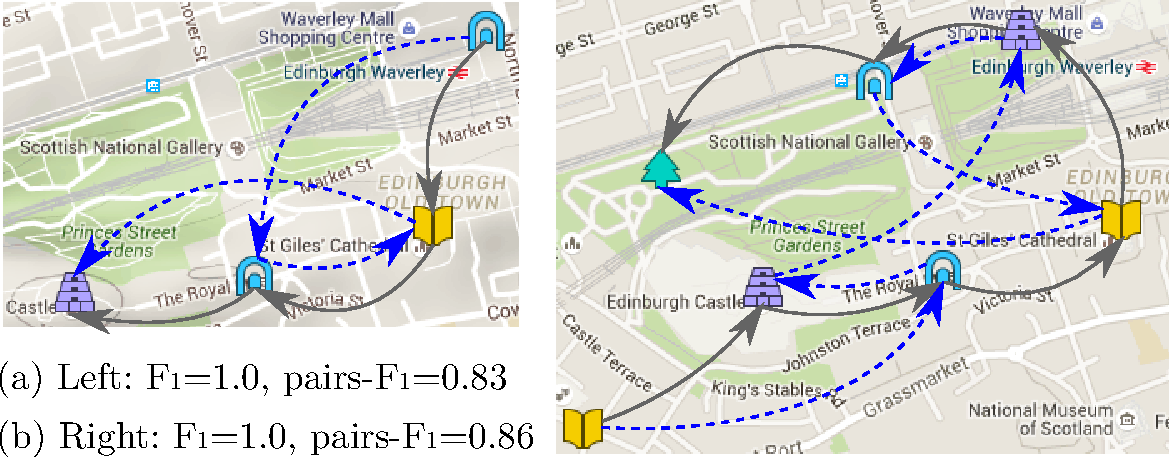
\includegraphics[width=\columnwidth]{fig/pairF1.pdf}
	\caption{Two illustrative examples for $F_1$ vs pairs-$F_1$ as evaluation metric for trajectories. Solid grey: ground truth trajectories; dashed blue: recommended trajectories.
    See Section~\ref{sec:metric} for details.}
	\label{fig:pairf1}\captionmoveup
\end{figure}


%To evaluate the performance of different trajectory recommendation algorithms,
%we employ the trajectory F$_1$\cite{ijcai15} to measure the POIs that are
%correctly recommended.
A commonly used metric for POI recommendation and evaluating trajectories is
the F$_1$ score on points.
Let $\mathcal{T}$ be the trajectory that was visited in the real world,
and $\hat{\cal T}$ be the recommended trajectory,
$\mathcal{P}_{\mathcal{T}}$ be the set of POIs visited in $\mathcal{T}$,
and $\mathcal{P}_{\hat{\mathcal{T}}}$ be the set of POIs visited in $\hat{\mathcal{T}}$,
we compute trajectory F$_1$ as the harmonic mean between the point-wise precision and recall.
%was defined as
\begin{displaymath}
F_1= \frac{2  P_{\textsc{point}}  R_{\textsc{point}}}
          {P_{\textsc{point}} + R_{\textsc{point}}}
\end{displaymath}
where
\vspace{-1.1em}
\begin{displaymath}%\eqmoveup
P_{\textsc{point}} = \frac{|\mathcal{P}_{\mathcal{T}} \cap \mathcal{P}_{\hat{\mathcal{T}}}|}
                          {|\hat{\mathcal{T}}|},
R_{\textsc{point}} = \frac{|\mathcal{P}_{\mathcal{T}} \cap \mathcal{P}_{\hat{\mathcal{T}}}|}
                          {|\mathcal{T}|}
\end{displaymath}

A perfect trajectory F$_1$ (i.e., F$_1 = 1$) means the POIs in
the recommended trajectory are exactly the same POIs as those in the ground truth,
and F$_1 = 0$ means that none of the POIs in the
real trajectory was recommended.

While trajectory F$_1$ is good at measuring whether POIs are correctly recommended,
it ignores the visiting order between POIs.
%Two trajectories with the exactly same set of POIs can be completely different to visitors
%given different routes.
An illustration is shown in Figure~\ref{fig:pairf1},
the solid grey lines represent the ground truth transitions that actually visited by travellers
and the dashed blue lines are the recommended trajectory by one of the approaches listed
in Table~\ref{tab:algsummary}. Both examples have a perfect F$_1$ score, but not a perfect
pairs-F$_1$ score due to the difference in POI sequencing.
%Even with the exactly same set of places, the visiting experiences are completely different because
%of the dramatically disparate routes.
%Enlightened by this observation,
We propose a new metric $\text{pairs-F}_1$ that takes into account
both the point identity and the visiting orders in a trajectory.
This is done by measuring the F$_1$ score of every pair of ordered POIs, whether they are adjacent or not.
\begin{displaymath}
\text{pairs-F}_1 = \frac{2 P_{\textsc{pair}} R_{\textsc{pair}}}
                       {P_{\textsc{pair}} + R_{\textsc{pair}}}
\end{displaymath}
where
\vspace{-2.0em}
\begin{displaymath}%\eqmoveup
~~
P_{\textsc{pair}} = \frac{N_c} {|\hat{\mathcal{T}}|(|\hat{\mathcal{T}}|-1) / 2}, ~
R_{\textsc{pair}} = \frac{N_c} {|\mathcal{T}|(|\mathcal{T}|-1) / 2}
\end{displaymath}
and $N_c$ is the number of ordered POI pairs $(p_j, p_k)$ that
appear in both the ground-truth and the recommended trajectories.
%satisfies the following
%conditions\footnote{We define pairs-F$_1=0$ if $N_c$ is $0$.}:
\begin{align*}
    (p_j \prec_{\mathcal{T}} p_k ~\land~ p_j \prec_{\hat{\mathcal{T}}} p_k)  ~\lor~
    (p_j \succ_{\mathcal{T}} p_k ~\land~ p_j \succ_{\hat{\mathcal{T}}} p_k) 
\end{align*}
with $p_j \ne p_k, ~p_j, p_k \in \mathcal{P}_{\mathcal{T}} \cap \mathcal{P}_{\hat{\mathcal{T}}}, ~1 \le j \ne k \le |\mathcal{T}|$.
Here $p_j \prec_{\mathcal{T}} p_k$ denotes POI $p_j$ was visited before POI $p_k$ in $\mathcal{T}$
and $p_j \succ_{\mathcal{T}} p_k$ denotes $p_j$ was visited after $p_k$ in $\mathcal{T}$.

Pairs-F$_1$ takes values between 0 and 1. A perfect pairs-F$_1$ (1.0) is achieved if and only if
both the POIs and their visiting orders in the
recommended trajectory are exactly the same as those in the ground truth.
Pairs-F$_1 = 0$ means none of the recommended POI pairs was actually visited in the real trajectory.


\subsection{Experimental setup}
\label{sec:setup}
\secmoveup
%


\begin{table}[t]
\caption{Summary of information captured by different trajectory recommendation algorithms}
\label{tab:algsummary}
\centering
%\small
\setlength{\tabcolsep}{3pt} % tweak the space between columns
\begin{tabular}{l|*{5}{c}} \hline
                                & Query    & POI      & Trans.     & No sub-      & Joint    \\
                                &          &          &            & tours        &          \\ \hline
\textsc{Random}                 & $\times$ & $\times$ & $\times$   & $\times$     & $\times$ \\
\textsc{PersTour}\cite{ijcai15} & $\times$ & $\surd$  & $\times$   & $\surd$      & $\times$ \\
\textsc{PersTour-L}             & $\times$ & $\surd$  & $\times$   & $\surd$      & $\times$ \\
\textsc{PoiPopularity}          & $\times$ & $\surd$  & $\times$   & $\times$     & $\times$ \\
\textsc{PoiRank}                & $\surd$  & $\surd$  & $\times$   & $\times$     & $\times$ \\
\textsc{Markov}                 & $\times$ & $\surd$  & $\surd$    & $\times$     & $\times$ \\
\textsc{MarkovPath}             & $\times$ & $\surd$  & $\surd$    & $\surd$      & $\times$ \\
\textsc{Rank+Markov}            & $\surd$  & $\surd$  & $\surd$    & $\times$     & $\times$ \\
\textsc{Rank+MarkovPath}        & $\surd$  & $\surd$  & $\surd$    & $\surd$      & $\times$ \\
\textsc{StructuredSVM}          & $\surd$  & $\surd$  & $\surd$    & $\times$     & $\surd$  \\ \hline
\end{tabular}
\captionmoveup
\end{table}

%
\begin{table*}[t]
\caption{Performance comparison on five datasets in terms of trajectory F$_1$ score.
         The best method for each dataset (i.e., a column) is shown in bold, the second best is shown in italic.}
\label{tab:f1}
\centering
\begin{tabular}{l|ccccc} \hline
 & Edinburgh & Glasgow & Melbourne & Osaka & Toronto \\ \hline
\textsc{Random} & $0.570\pm0.139$ & $0.632\pm0.124$ & $0.558\pm0.149$ & $0.621\pm0.117$ & $0.621\pm0.128$ \\
\textsc{PersTour}\cite{ijcai15} & $0.656\pm0.223$ & $\mathbf{0.802\pm0.213}$ & $0.491\pm0.211$ & $0.702\pm0.230$ & $0.720\pm0.215$ \\
\textsc{PersTour-L} & $0.651\pm0.143$ & $0.660\pm0.102$ & $0.578\pm0.140$ & $0.691\pm0.138$ & $0.642\pm0.112$ \\
\textsc{PoiPopularity} & $\mathbf{0.701\pm0.160}$ & $0.745\pm0.166$ & $0.621\pm0.136$ & $0.661\pm0.128$ & $0.679\pm0.120$ \\
\textsc{PoiRank} & $\mathit{0.694\pm0.157}$ & $\mathit{0.777\pm0.171}$ & $\mathbf{0.626\pm0.137}$ & $0.679\pm0.112$ & $\mathbf{0.748\pm0.166}$ \\
\textsc{Markov} & $0.629\pm0.172$ & $0.714\pm0.168$ & $0.577\pm0.168$ & $0.679\pm0.162$ & $0.663\pm0.157$ \\
\textsc{MarkovPath} & $0.678\pm0.148$ & $0.735\pm0.170$ & $0.596\pm0.147$ & $0.706\pm0.154$ & $0.689\pm0.140$ \\
\textsc{Rank+Markov} & $0.642\pm0.171$ & $0.736\pm0.176$ & $0.598\pm0.169$ & $0.701\pm0.171$ & $0.689\pm0.170$ \\
\textsc{Rank+MarkovPath} & $0.684\pm0.151$ & $0.760\pm0.170$ & $\mathit{0.625\pm0.150}$ & $\mathbf{0.719\pm0.161}$ & $0.724\pm0.152$ \\
%\textsc{StructuredSVM} & $0.659\pm0.186$ & $0.727\pm0.173$ & $0.597\pm0.171$ & $\mathit{0.715\pm0.170}$ & $\mathit{0.728\pm0.186}$ \\
\hline
\end{tabular}\captionmoveup
\end{table*}


\begin{table*}[t]
\caption{Performance comparison on five datasets in terms of pairs-F$_1$.
         The best method for each dataset (i.e., a column) is shown in bold, the second best is shown in italic.}
\label{tab:pairf1}
\centering
\begin{tabular}{l|ccccc} \hline
 & Edinburgh & Glasgow & Melbourne & Osaka & Toronto \\ \hline
\textsc{Random} & $0.261\pm0.155$ & $0.320\pm0.169$ & $0.249\pm0.148$ & $0.305\pm0.145$ & $0.311\pm0.167$ \\
\textsc{PersTour}\cite{ijcai15} & $0.417\pm0.343$ & $\mathbf{0.646\pm0.366}$ & $0.225\pm0.274$ & $\mathit{0.491\pm0.377}$ & $0.503\pm0.353$ \\
\textsc{PersTour-L} & $0.359\pm0.207$ & $0.352\pm0.162$ & $0.268\pm0.143$ & $0.415\pm0.243$ & $0.331\pm0.159$ \\
\textsc{PoiPopularity} & $\mathit{0.436\pm0.259}$ & $0.509\pm0.299$ & $0.316\pm0.178$ & $0.363\pm0.195$ & $0.385\pm0.202$ \\
\textsc{PoiRank} & $0.424\pm0.249$ & $\mathit{0.565\pm0.312}$ & $0.322\pm0.186$ & $0.376\pm0.173$ & $\mathit{0.512\pm0.295}$ \\
\textsc{Markov} & $0.424\pm0.238$ & $0.488\pm0.283$ & $0.297\pm0.192$ & $0.449\pm0.262$ & $0.419\pm0.237$ \\
\textsc{MarkovPath} & $0.400\pm0.234$ & $0.492\pm0.298$ & $0.294\pm0.187$ & $0.445\pm0.268$ & $0.407\pm0.234$ \\
\textsc{Rank+Markov} & $0.434\pm0.251$ & $0.540\pm0.294$ & $\mathbf{0.357\pm0.210}$ & $0.483\pm0.277$ & $0.462\pm0.266$ \\
\textsc{Rank+MarkovPath} & $0.408\pm0.239$ & $0.532\pm0.304$ & $0.331\pm0.213$ & $0.470\pm0.284$ & $0.465\pm0.266$ \\
%\textsc{StructuredSVM} & $\mathbf{0.440\pm0.267}$ & $0.529\pm0.283$ & $\mathit{0.352\pm0.213}$ & $\mathbf{0.508\pm0.292}$ & $\mathbf{0.520\pm0.311}$ \\
\hline
\end{tabular}\captionmoveup
\end{table*}

%
\begin{figure*}[t]
	\centering
	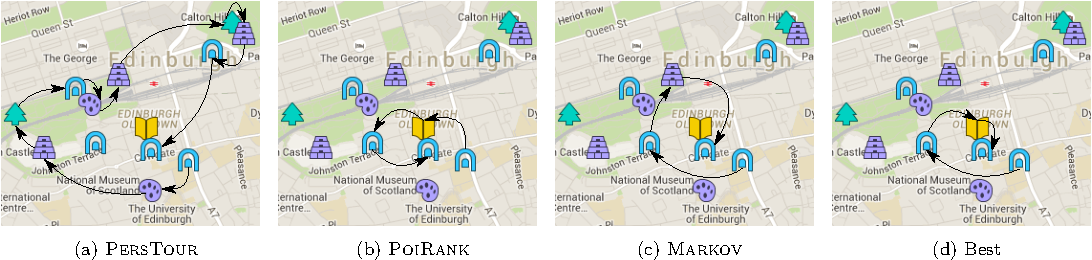
\includegraphics[width=\textwidth]{fig/example-tour.pdf}
	\caption{Different recommendations from algorithm variants.
    See the main text in Section~\ref{sec:example} for description.}
	\label{fig:exampleresult}
	\captionmoveup
\end{figure*}

We use leave-one-out cross validation to evaluate different trajectory recommendation algorithms,
i.e., when testing on a trajectory, all other trajectories are used for training.
We compare with a number of baseline approaches from recent literature, the 10 variants of approaches
are summarised below, with an overview in Table~\ref{tab:algsummary}.

% baseline: Random, PersTour, PersTour-L, PoiPopularity
{\bf Baseline approaches} including \textsc{Random} which naively chooses POIs uniformly at random
(without replacement) from the set of POIs $\mathcal{P} \setminus \{p_s, p_e \}$ to form a trajectory.
It does not utilise any features related to POI or query, as shown in Table~\ref{tab:algsummary}.
Among the related approaches, \textsc{PersTour}~\cite{ijcai15} is the most similar work and it
explores both POI features and the sub-tour elimination constraints described in Section~\ref{sec:walkpath},
in addition, the recommended trajectory is constrained by a time budget.
One variant of \textsc{PersTour} is applying the trajectory length instead of the time budget to constrain
the recommended trajectory, which is denoted as \textsc{PersTour-L} in Table~\ref{tab:algsummary}.
Another baseline is \textsc{PoiPopularity} described at the beginning of Section~\ref{sec:method},
it only uses POI popularity to recommend a trajectory.

% variants: PoiRank, Markov, MarkovPath, Rank+Markov, Rank+MarkovPath, SSVM
{\bf Variants of point- and route-ranking} approaches including \textsc{PoiRank} (Section~\ref{sec:ranksvm})
that utilises POI and query features,
and \textsc{Markov} (Section~\ref{sec:transition}),
that recommends trajectories uses only transition probabilities between POIs
and its variant \textsc{MarkovPath} that incorporates additional constraints to eliminate sub-tours.
Both \textsc{Rank+Markov} and \textsc{Rank+MarkovPath} (Section~\ref{sec:rank+markov})
utilise POI and query features as well as transition probabilities, with the latter uses
additional sub-tour elimination constraints.
%Lastly, we have the \textsc{StructuredSVM} (Section~\ref{sec:ssvm}) that not only utilises POI and query features
%as well as transition probabilities but also jointly optimises their relative importance.

% Parameters
{\bf Parameters} of these algorithms.
We use a $0.5$ trade-off parameter for \textsc{PersTour} and \textsc{PersTour-L},
found to be the best weighting by \textsc{PersTour}~\cite{ijcai15}.
We set the regularisation parameter in rankSVM to  $10.0$, determined by cross-validation.
The trade-off value in \textsc{Rank+Markov} and \textsc{Rank+MarkovPath} is also $0.5$.
% and the regularisation parameter in \textsc{StructuredSVM} is $1.0$.


\subsection{Results}
\label{sec:result}
\secmoveup

% compare both F1 and pair F1 at the same time
The performance of the baseline algorithm and the POI ranking and routing variants
on five trajectories datasets are summarised in Table~\ref{tab:f1}
and Table~\ref{tab:pairf1}, in terms of trajectory F$_1$ score and pairs-F$_1$, respectively.

% 6. xxPath vs. xx:
% MarkovPath vs Markov:
% in terms of F1, MarkovPath (Rank+MarkovPath) is always better than Markov (Rank+Markov),
% in terms of pair F1, MarkovPath (Rank+MarkovPath) yields comparable or worse performance than Markov.
% which indicates that sub-tour elimination helps POI prediction but worsen the visiting order.

We can see from Table~\ref{tab:f1} that \textsc{MarkovPath} and \textsc{Rank+MarkovPath}
outperform their corresponding variants \textsc{Markov} and \textsc{Rank+Markov} without the path constraints in terms of F1.
This demonstrates that eliminating sub-tours improves point recommendation.
This is expected, as sub-tours worsen the proportion of correctly
recommended POIs since a length constraint is used.
On the contrary, most Markov chain entries have better performance in terms of pairs-F$_1$
which indicates Markov chain approaches generally
respect the transition patterns between POIs.
% go to SSVM
%The effect of sub-tours on trajectory recommendation can be further observed through the performance of \textsc{StructuredSVM}.
%
% 7. SSVM vs Rank+Markov and Rank+MarkovPath:
% while SSVM using the same features as Rank+Markov and Rank+MarkovPath, and took advantage of its significantly larger number of parameters
% but SSVM permit sub-tours
% in terms of F1,
% it either yield comparable performance with the better performer (Osaka/Toronto) or with the worse performer (Edinburgh/Glasgow/Melbourne)
% which indicate how hurt sub-tours hurts POI recommendation.
% on the other hand, in terms of pair F1.
% it takes advantage of the transition patterns and yields comparable (Glasgow/Melbourne) or better performance than both of them
While utilising the same features as \textsc{Rank+Markov} and \textsc{Rank+MarkovPath},
it is more flexible with automatic tuning of the trade-off of points and routes, resulting in
the best performance with respect to pair-F1 in Edinburgh, Osaka and Toronto.
%it can further take advantage of the significantly larger number of parameters.
%However, \textsc{StructuredSVM} can only yield comparable performance with the best performer
%among the three at most, when measured in terms of trajectory F$_1$.
%While not achieving best point F1 in any city,
%\textsc{StructuredSVM} makes the best use of transition patterns
%and consistently has better pairs-F1 than \textsc{Rank+Markov} and \textsc{Rank+MarkovPath} in all cities.
%which leads to comparable or
%better performance, in terms of pairs-F$_1$, than both of them all the time.
%This observation is consistent with the effect of sub-tours observed above
%as \textsc{StructuredSVM} does permit the existence of sub-tours in recommended trajectories.


% go to ranking based algorithms
Algorithms based on POI rankings yield strong performance
by exploring POI and query specific features.
%
% 3. PoiRank vs. PoiPopularity
% PoiRank yields nice improvement on four datasets, only slightly downgraded on Edinburgh
%\textsc{PoiPopularity} baseline performs pretty well despite its simplicity,and
\textsc{PoiRank} improves notably upon \textsc{PoiPopularity} and \textsc{PersTour}
 by leveraging more POI features and query specific features in 3 out of 5 datasets.
%except slightly worse on Edinburgh dataset on which \textsc{PoiPopularity} is the best and
%second best performer in terms trajectory F$_1$ and pairs-F$_1$ respectively.
% go to transition based algorithms
On the other hand, Algorithm that leverage transition probabilities alone does not perform particularly well.
%
% 4. PoiRank vs. Markov:
% in terms of F1, PoiRank always performs much better, except on Osaka where both yield comparable performance
In terms of trajectory F$_1$,
\textsc{Markov} can not outperform \textsc{PoiRank} except on Osaka dataset,
on which the performance of both algorithms are comparable.
In particular, algorithms with ranking information (e.g. \textsc{Rank+Markov} and \textsc{Rank+MarkovPath}) 
always out-perform their respective variants with transition information alone (i.e. \textsc{Markov} and \textsc{MarkovPath}).

% in terms of pair F1, PoiRank is significantly better on Glasgow, Melbourne and Toronto, comparable on Edinburgh
\textsc{PoiRank} performs significantly better than \textsc{Markov} on three datasets, namely,
Glasgow, Melbourne and Toronto.
%
% at the first sight, it seems strange because Markov modelled the transitions and pair F1 measures the visiting order
% but actually pair F1 is affected heavily by the number of correctly predicted POIs, once the POIs are correctly predicted, it will yield
% better pair F1, this is consistent with the observation that, on Osaka dataset, Markov and PoiRank yield comparable F1,
% but Markov outperforms PoiRank significantly in terms of pair F1.
This result may seem strange at first sight because \textsc{Markov} modelled the transition patterns and it could leverage
this advantage to accomplish better performance in terms of pairs-F$_1$ given the fact that this metric is measuring the quality
of visiting order.
However, pairs-F$_1$ is actually affected heavily by the proportion of correctly recommended POIs in trajectory,
once the POIs are correctly predicted, a better pairs-F$_1$ would be achieved,
this supposition can be confirmed by the observation that, on Osaka dataset, \textsc{Markov} and \textsc{PoiRank} achieved
comparable performance in terms of trajectory F$_1$, which means the proportion of correctly recommended POIs is comparable,
but \textsc{Markov} outperforms \textsc{PoiRank} significantly in terms of pairs-F$_1$,
which suggest the transition information is helpful in some situations.

% 5. PoiRank vs. Markov vs. Rank+Markov
% in terms of both F1 and pair F1,
% when the advantage of PoiRank over Markov is large, Rank+Markov always brings improvements on Markov, but can't compete with PoiRank
% as the advantage gap of PoiRank over Markov shrinks, performance of Rank+Markov becomes closer to PoiRank,
% when the Markov is comparable or better than PoiRank, Rank+Markov outperforms both (Osaka)
% which is consistent with the assumption that transition helps when ranking didn't performs very well
Transition information helps point ranking when their performances are comparable.
When the advantage gap of \textsc{PoiRank} over \textsc{Markov} is large,
i.e. Edinburgh, Glasgow, Melbourne and Toronto in Table~\ref{tab:f1} and Glasgow, Toronto in Table~\ref{tab:pairf1},
transition information does not help \textsc{Rank+Markov}, which explores both POI ranking and transitions,
can not compete with \textsc{PoiRank} in both metrics, but nevertheless brings improvements to \textsc{Markov}.
However, as the performance of \textsc{Markov} approaches or surpasses that of \textsc{PoiRank},
i.e., Osaka in Table~\ref{tab:f1} and Edinburgh, Melbourne, Osaka in Table~\ref{tab:pairf1},
\textsc{Rank+Markov} outperforms both of them, this observation indicates that transition information can be very helpful when
ranking does not performs well enough.


% Baseline stuff, move to the end
% always better than Random, except PersTour on Melbourne which we'll illustrate later
\textsc{PersTour}~\cite{ijcai15} always performs better than its variant \textsc{PersTour-L},
especially on Glasgow and Toronto datasets.
This indicate the time budget constraint is more helpful than length constraint for recommending trajectories.
The exception on Melbourne dataset is explained next.
It is obvious that algorithms captured a certain type of information as shown in Table~\ref{tab:algsummary}
outperforms the \textsc{Random} baseline in terms of both performance metrics on all five datasets,
except the performance of \textsc{PersTour}\cite{ijcai15} on Melbourne dataset which will be interpreted later.
% 2. PersTour vs. PersTour-L
% PersTour always better except on Melbourne which analysed later
%where the advantage gap of \textsc{PersTour}
%is significantly large in terms of both performance metrics,
%
% brief mention results of algorithms with and without utilising time budget constraint

% 8. PersTour on Melbourne:
% we observed that PersTour was outperformed by Random on Melbourne dataset in terms of both F1 and pair F1.
% it turns out on Melbourne dataset, the many of the ILPs which PersTour solve to get the recommendation result are very hard ILP instances
% in the leave-one-out evaluation, although we utilise a large scale computing cluster with modern hardware,
% there are 12\% of evaluations are failed due to ILP solver can't find a feasible solution in a $2$ hours
% furthermore, a lot recommendations are suboptimal solutions of the ILP due to the $2$ timeout settings.
% which leads to PersTour, which is always a strong performer on other datasets, performs inconsistently on Melbourne dataset.
Lastly, we observed that \textsc{PersTour} is surprisingly outperformed by \textsc{Random} baseline
on Melbourne dataset in terms of both metrics.
It turns out that, on this very dataset, many of the integer linear programming (ILP) problems
which \textsc{PersTour} need to solve to get the recommendations are difficult ILP instances.
In the leave-one-out evaluation, although we utilised a large scale computing cluster with modern hardware,
$12\%$ of evaluations failed due to the ILP solver could not find a feasible solution in $2$ hours.
Furthermore, a lot of recommendations are produced from suboptimal solutions of the corresponding ILPs due to
the $2$ hours timeout setting, these factors lead to the inconsistent performance of \textsc{PerTour} on Melbourne dataset.


\subsection{Example}
\label{sec:example}
\secmoveup

Figure~\ref{fig:exampleresult} illustrates a test case in Edinburgh dataset.
The ground truth is a trajectory of length $4$ that starts at a POI of category \textit{Structures},
visits two intermediate POIs of category \textit{Structures} and \textit{Cultural} and
terminates on a POI of category \textit{Structures}.
The trajectory recommended by \textsc{PersTour} is a tour with $11$ POIs, as shown in Figure~\ref{fig:exampleresult}(a),
with none of the desired intermediate POIs visited.
\textsc{PoiRank} (Figure~\ref{fig:exampleresult}(b)) recommended a tour with correct POIs using
POI specific features (illustrated in Figure~\ref{fig:distro}) as well as query specific features,
but with completely different routes.
On the other hand, \textsc{Markov} (Figure~\ref{fig:exampleresult}(c)) missed one POI but the recommended route for one of the intermediate is consistent with the ground truth.
The best recommendation, as shown in Figure~\ref{fig:exampleresult}(d), with exactly the same points and routes as the ground truth,
which in this case is achieved by \textsc{Rank+MarkovPath}.





\section{Conclusion}
\label{sec:conclusion}
In this paper, we present an approach to utilize learning to rank as well as factorized Markov Chain to explore both
POI properties and transition patterns between POIs, then combine them using a probabilistic model and structured 
support vector machine to recommend trajectory. 
We evaluate the performance of our approach on four trajectory datasets extracted from Flickr photos using both 
trajectory F$_1$-score and trajectory $\tau$, experimental results show not only performance improvements over 
state-of-the-art methods but also many interesting properties of trajectories in different datasets.


%\section{Acknowledgments}
%We thank Kwan Hui Lim for kindly providing his R code to reproduce his experiments.

{\small
\bibliographystyle{abbrv}
\bibliography{ref}
}

\newpage
\appendix
\section{Details}
We collected the POI categories in all of the five trajectory datasets
and their names with the corresponding icons are shown in figure \ref{fig:poicats}.

Three POI features used to rank POIs, namely, the popularity,
the total number of visits and the visit duration, in all five datasets are shown in
figure \ref{fig:popularity}, figure \ref{fig:nvisit} and figure \ref{fig:duration} respectively.

Figure \ref{fig:transmat} shows the heat map of the transition matrices for $5$ individual POI features
in Melbourne dataset.

\begin{table}
\caption{Statistics of trajectory dataset}
\label{tab:data}
\centering\small
\begin{tabular}{lrrrrr} \hline
\textbf{Dataset} & \textbf{\#Photos} & \textbf{\#Visits} & \textbf{\#Traj.} & \textbf{\#Users} \\ \hline
Edinburgh & 82,060 & 33,944 & 5,028 & 1,454 \\
Glasgow & 29,019 & 11,434 & 2,227 & 601 \\
Melbourne & 94,142 & 23,995 & 5,106 & 1,000 \\
Osaka & 392,420 & 7,747 & 1,115 & 450 \\
Toronto & 157,505 & 39,419 & 6,057 & 1,395 \\
\hline
\end{tabular}
\end{table}


%\begin{figure}
%\centering
%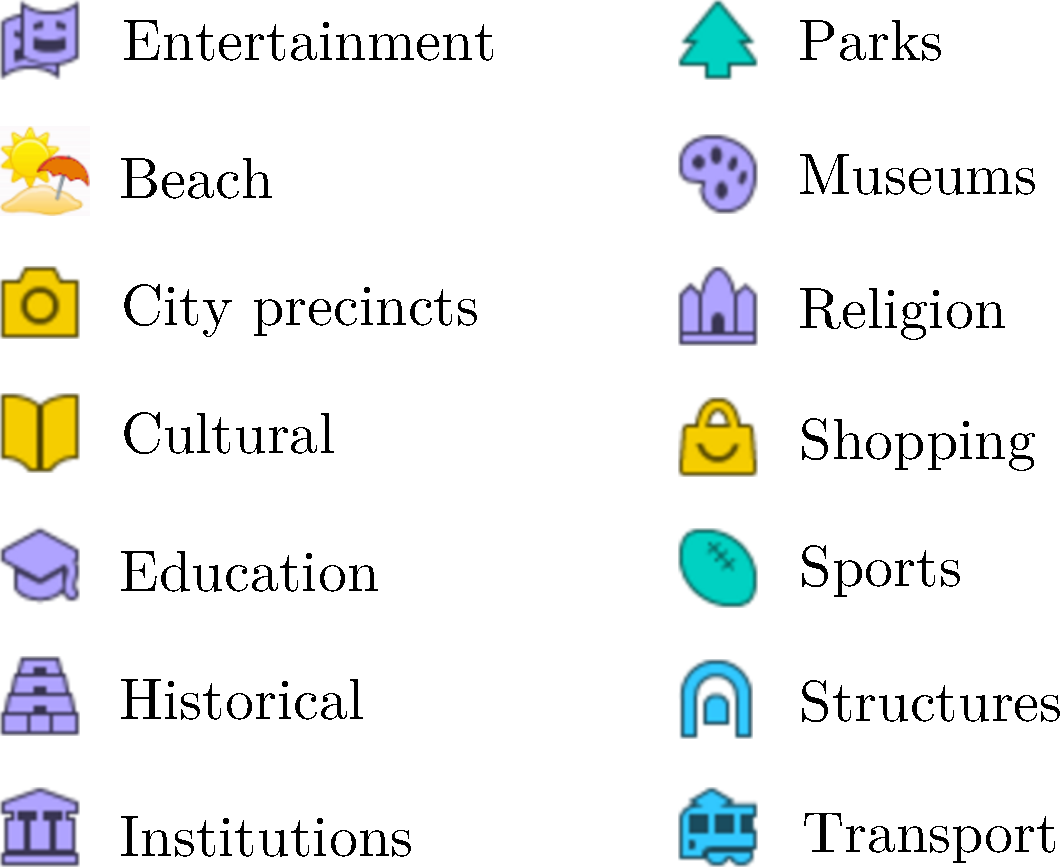
\includegraphics[width=\columnwidth]{fig/poi_cats.pdf}
%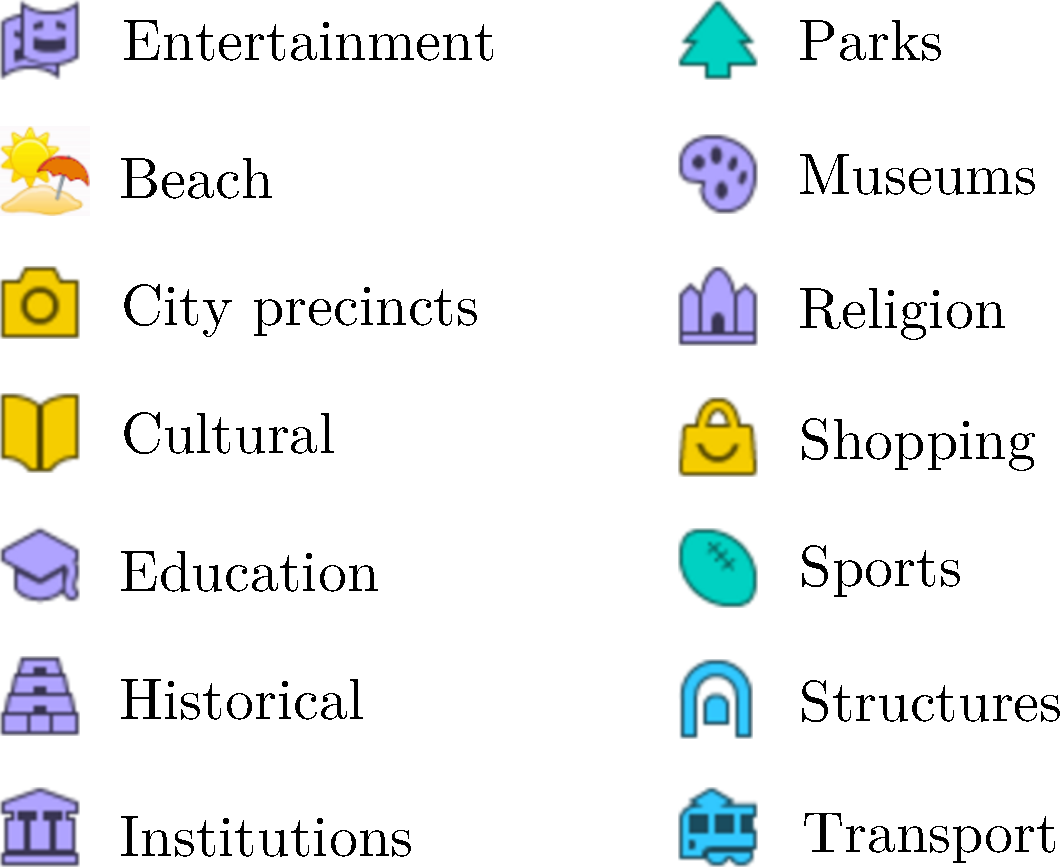
\includegraphics[scale=.32]{fig/poi_cats.pdf}
%\caption{POI categories}
%\label{fig:poicats}
%\end{figure}

\begin{figure*}[t]
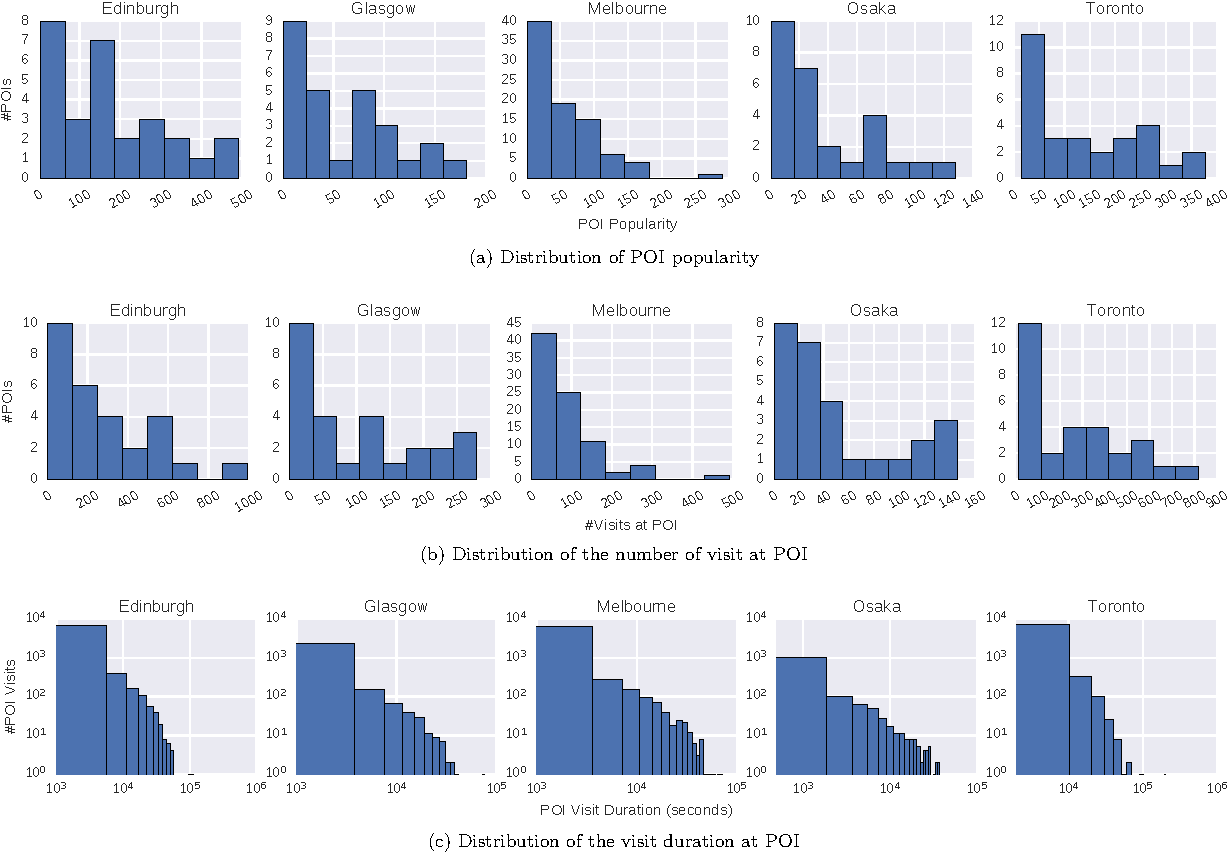
\includegraphics[width=\textwidth]{fig/feature_distro.pdf}
\caption{Distribution of POI popularity, the number of visit and visit duration}
\label{fig:distro}
\end{figure*}

\cheng{Report the proportion of recommended trajectories and actual trajectories with sub-tours, in the Appendix.}

\section{POIs with same features}


By computing the Kronecker product of transition matrices of all the POI features,
we get an unnormalised transition matrix of POI features.
However, to obtain the transition probabilities between each POI pair $(p_i, p_j)$,
there are two cases needs to be dealt with properly:
\begin{enumerate}
\item POI features which represent POIs that do not exist in $\mathcal{P}$,
\item POI features that corresponds to more than one POIs in $\mathcal{P}$.
\end{enumerate}

% deal with feature vector without corresponding POI or with more than one POIs.
For the first case,
the corresponding rows and columns in the result matrix of Kronecker product are simply removed.

The second case was a bit subtle.
Let POIs with exactly the same features be a POI group,
the transition probabilities associated with POIs in the same group are computed as follows:
\begin{itemize}
\item The incoming (unnormalised) transition probability of the group was divided uniformly among POIs
      in the same group, which is equivalent to choose a POI in the group uniformly at random;
\item The outgoing (unnormalised) transition probability of each POI should be the same as the
      outgoing transition probability of the POI group, as one had already been in the POI group in this case;
\item The self-loop of the POI group represents the transitions between POIs in the same group,
      suppose the (unnormalised) transition probability from a POI group to itself is $P_o$,
      and the number of POIs in the group is $N_o$,
      the transition probability from $p_i$ to $p_j$ in the same group is
      \begin{displaymath}
          P(p_j | p_i) =
          \begin{cases}
              \hfill 0, \hfill & i = j \\
              \hfill \frac{P_o}{N_o - 1}, \hfill & i \ne j \\
          \end{cases}
      \end{displaymath}
\end{itemize}
Finally, the unnormalised outgoing transition probabilities of each POI were normalized to form
a valid probability distribution
\footnote{Note that dealing with the second case before or after the normalization leads to
the same transition probabilities, which can be easily proved. \cheng{Show proof}}.


\section{Avoid Peeking}
When working with machine learning algorithms, to make sure the reported performance is a good approximation
of the generalization performance, it is critical to prevent information in test set from leaking into
training set.
Many algorithms in the above comparison utilizing both learning to rank and factorized transition matrix,
e.g., \textsc{Rank+Markov}, \textsc{Rank+MarkovPath} and \textsc{StructuredSVM},
both of them need to be trained or parameters be estimated before being utilized in other algorithms.
Features such as popularity of a POI, the number of visits of a POI and the average visit duration at a POI are
determined by not only the POI itself but also trajectories in training set, let's call them aggregated features as they are
computed by aggregating a set of trajectories.
To make sure the prediction performance is reliable, it is very important to exclude trajectories in test set
when computing aggregated features.
Unfortunately, it is quite easy, especially when utilizing multiple levels of machine learning models,
to use all data, including those in test set, to compute aggregated features and many researchers and
practitioners did not realize some bits of information in test set were leaked into training set via these aggregated features.

%One may argue that many of these features will not change much when computed with or without data in test set,
%but in certain areas, such as aerodynamics, some decisions are very sensitive to the quantity of certain features.
%Nevertheless, the exact impact still needs further investigation.

\section{Implementation details}
libsvmtools, PyStruct, Gurobi, etc.

There are about $12$\% of trajectories in Melbourne dataset that were failed to be evaluated
using \textsc{PersTour} due to the timeout of integer programming solver, the timeout is $2$ hours.


\end{document}
